\documentclass[preprint,review,12pt]{elsarticle}

\usepackage{amsmath,amsfonts,amssymb}
\usepackage{booktabs}
\usepackage{longtable}
\usepackage{url}
\usepackage{makecell}
\usepackage{flafter}
\usepackage{placeins}
\usepackage{float}
\usepackage{multirow}
\usepackage{subcaption}
\usepackage{hyperref}

\hypersetup{
  pdftitle={Transform Ordering and Selection in Convolutional Neural Network Preprocessing for Binary Skin Image Classification},
  pdfauthor={Gabriel Mitelman Tkacz and Gustavo Scalabrini Sampaio and Leandro Augusto da Silva},
  colorlinks=true,
  linkcolor=blue,
  citecolor=blue,
  urlcolor=blue,
}

\hyphenation{op-tical net-works semi-conduc-tor pre-proc-ess-ing der-ma-to-log-i-cal}

\journal{Computers in Biology and Medicine}
\setlength{\emergencystretch}{3em}

\begin{document}

\begin{frontmatter}

\title{Transform Ordering and Selection in Convolutional Neural Network Preprocessing for Binary Skin Image Classification}

\author[ee]{Gabriel Mitelman Tkacz\corref{cor1}}
\ead{gabriel@tkacz.dev.br}
\ead[url]{https://orcid.org/0009-0004-3619-4561}

\author[fci]{Gustavo Scalabrini Sampaio}
\ead{gustavo.sampaio@mackenzie.br}
\ead[url]{https://orcid.org/0000-0003-1150-5584}


\author[fci]{Leandro Augusto da Silva}
\ead{leandroaugusto.silva@mackenzie.br}
\ead[url]{https://orcid.org/0000-0002-8671-3102}

\cortext[cor1]{Corresponding author.}

\affiliation[ee]{organization={School of Engineering, Mackenzie Presbyterian University},
            addressline={Rua da Consola\c{c}\~ao, 930},
            city={S\~ao Paulo},
            state={SP},
            postcode={01302-907},
            country={Brazil}}

\affiliation[fci]{organization={Faculty of Computing and Informatics, Mackenzie Presbyterian University},
            addressline={Rua da Consola\c{c}\~ao, 930},
            city={S\~ao Paulo},
            state={SP},
            postcode={01302-907},
            country={Brazil}}

\begin{abstract}
Preprocessing transforms are often combined without testing whether their order changes downstream model performance. We evaluated all 65 pipelines formed by applying each of four concrete transform implementations at most once: histogram equalization, fixed affine normalization, bilateral filtering, and RGB-to-HSV conversion. A four-block convolutional neural network was trained from scratch for every pipeline under five random seeds on a balanced, cross-source healthy-versus-diseased skin-image dataset containing 12{,}078 images. The unprocessed baseline reached 98.09\% mean test accuracy. Equalization alone had a positive mean gain of $+0.22$ percentage points (95\% bootstrap CI $[-0.07,+0.50]$), while all 60 multi-transform pipelines had negative mean gains. Pipeline length correlated with mean accuracy gain ($r=-0.44$, Holm-adjusted $p=0.0013$). At length three, transform selection accounted for 42\% of the observed variance and ordering for 58\%. Pipelines with equalization first were 1.10 percentage points less harmful on average than the pooled alternatives, and the equalization-first, normalization-last bookend was 2.00 percentage points less harmful than its reverse. At the fixed decision threshold, both false-positive and false-negative counts increased for 50 of 64 non-baseline pipelines. This sign pattern does not by itself distinguish feature loss from miscalibration. A linear probe using only global color statistics reached 93.4\% accuracy, consistent with the strong source/class confound built into the dataset. The results establish order sensitivity for these implementations and value-range conventions. They support a range-aware harm-minimization rule within this experiment, not a general clinical preprocessing prescription.
\end{abstract}

\begin{keyword}
Image preprocessing \sep transform ordering \sep preprocessing pipeline design \sep convolutional neural networks \sep medical image classification \sep skin image classification
\end{keyword}

\end{frontmatter}

\section{Introduction}
Artificial-intelligence tools are increasingly used to support dermatologic diagnosis, particularly in computer-aided diagnosis (CADx) systems trained on dermatoscopic and clinical images~\cite{Krakowski2024}. Deep learning models have achieved dermatologist-level performance on skin-lesion classification~\cite{Esteva2017, Brinker2019} and improved primary-care clinicians' accuracy in assisted teledermatology triage~\cite{10.1001/jamanetworkopen.2021.7249}. Reported performance also depends on the quality and preparation of the input images~\cite{ALHINAI20201, Brinker2019}.

Image preprocessing applies transforms such as normalization, histogram equalization, denoising, and color-space conversion before model ingestion~\cite{RODRIGUES2020103542, 9548351, Tarawneh2024}. Pipelines are often built by selecting transforms thought to help individually and ordering them by convention or intuition. A typical workflow might normalize intensity values, reduce noise, and enhance contrast without directly testing alternative orders.

This conventional approach makes transform selection the main design decision and often treats ordering as either unimportant or inferable from the stated purpose of each operation. Few medical-image studies have measured selection and ordering separately across a complete, fixed transform set. In practice, composed implementations may be non-commutative for two reasons. The mathematical operations can depend on the input distribution, and their software implementations can impose value-range and color-space contracts that make the output of one transform a poor input to another.

We address this gap by evaluating every ordered pipeline formed from four image transforms used at most once: histogram equalization~(E), intensity normalization~(N), bilateral denoising~(D), and color-space conversion~(CS). The design covers every permutation at lengths one through four, giving 64 non-baseline configurations and the unprocessed baseline. This complete matrix permits separate analysis of variation associated with transform selection and transform ordering.

Across five seeds per configuration, pipeline length correlates negatively with mean accuracy gain ($r=-0.44$, $p_{\mathrm{Holm}}=0.0013$), and none of the 60 multi-transform pipelines has a positive mean gain against the 98.09\% baseline. The variance point estimate changes from selection-dominated at $k=2$ ($\eta^2=0.76$, not significant after correction) to ordering-dominated at $k=3$, where ordering accounts for 58\% of observed variance ($\eta^2_{\text{selection}}=0.42$, $F(3,20)=4.83$, $p_{\mathrm{Holm}}=0.0245$). At $k=4$, all pipelines contain the same transforms, and the 24 orderings span 3.78 percentage points. Equalization performs better near the start and normalization near the end. The pooled equalization-first contrast has Cohen's $d=1.22$ ($p_{\mathrm{Holm}}=0.00055$), while the equalization-first, normalization-last bookend differs from its reverse by 2.00 percentage points ($d=2.38$, $p_{\mathrm{Holm}}=0.0245$). At the fixed decision threshold, both error counts rise for 78\% of non-baseline pipelines. This is a descriptive operating-point result and does not identify an irreversible feature-space mechanism without stored scores and a threshold sweep.

For these implementations, the least harmful recurring pattern is $\text{E} \to \{\text{D},\text{CS}\} \to \text{N}$. The pattern is consistent with the code's range contracts because equalization and color conversion clamp their inputs to $[0,1]$, while normalization can move values outside that interval. It is an implementation-specific result on a cross-source dataset, not evidence for a universal medical-image preprocessing order. Section~\ref{sec:related} reviews earlier preprocessing studies. Section~\ref{sec:methods} describes the experiment and statistical analysis. Sections~\ref{sec:results} and~\ref{sec:discussion} report and interpret the results, and Section~\ref{sec:conclusion} states the bounded conclusion.

\section{Related Work}
\label{sec:related}

Image preprocessing has been studied across several clinical domains, but prior work usually evaluates individual transforms rather than their combinatorial interactions~\cite{Koresh2024}.

Rodrigues~et~al.~\cite{RODRIGUES2020103542} evaluated six preprocessing strategies for HEp-2 cell classification in immunofluorescence images, including the unprocessed image, mean subtraction, contrast stretching, and histogram equalization. They reported the highest accuracy on unprocessed images for most CNN architectures, with Inception-V3 reaching 96.69\%; only ResNet-50 benefited from contrast stretching. Their study evaluated each strategy independently and did not examine multi-stage pipelines or transform ordering.

In biometric authentication, Tarawneh~et~al.~\cite{Tarawneh2024} investigated mean and median filtering for CNN-based dorsal hand vein recognition. They reported training accuracy rising from 70\% without preprocessing to 99\% with mean filtering. The study evaluated single transforms rather than their combinations or orderings.

For dermatoscopic image analysis specifically, deep learning has achieved dermatologist-level performance on skin cancer classification~\cite{Esteva2017}, motivating extensive work on preprocessing pipelines for this modality. Arora~et~al.~\cite{ARORA2021102358} proposed a modified U-Net architecture incorporating group normalization and attention gates for skin lesion segmentation, achieving segmentation accuracies of 95--97\% across four public databases. Dash~et~al.~\cite{DASH2020106240} developed a cascaded deep CNN framework for psoriasis severity assessment that included intensity normalization and artifact removal as preprocessing steps. Nugroho~et~al.~\cite{10810559} examined the effect of preprocessing, specifically hair removal, contrast enhancement, and noise reduction, on skin lesion segmentation accuracy, demonstrating that appropriate preprocessing improved segmentation performance. In each case, the preprocessing pipeline was designed and applied as a fixed sequence without systematic exploration of alternative orderings.

Av\c{s}ar~\cite{9548351} evaluated the effects of image preprocessing on CNN performance for pneumonia detection, testing preprocessing techniques including Wiener filtering and histogram equalization. The study demonstrated that preprocessing selection significantly affected classification accuracy, but, like the other works reviewed here, did not address the ordering of multi-stage pipelines. Vincent and Roopa Jayasingh~\cite{9780692} surveyed preprocessing techniques for psoriasis detection, cataloguing segmentation, feature extraction, and classification approaches without examining how the sequencing of these operations affects downstream accuracy.

The studies above mainly treat preprocessing transforms as individual interventions or use one fixed multi-stage sequence. We found no exhaustive ordering study for a fixed transform set in this medical-image setting. The present experiment evaluates all 65 configurations formed from four implementations and compares between-set variation, associated with transform selection, with within-set variation, associated with ordering.


\section{Methodology}
\label{sec:methods}

\subsection{Dataset and Classification Architecture}
\label{subsec:dataset}

The experimental dataset was constructed by combining dermatoscopic images of skin lesions from the HAM10000 collection~\cite{Tschandl2018, Codella2019} with images of healthy skin from the publicly available Healthy Skin Dataset~\cite{megpaulson_healthy_skin}, forming a class-balanced binary classification task comprising 12{,}078 images (6{,}039 diseased and 6{,}039 healthy). Because the two classes are drawn from different acquisition sources, a cross-source confound bears on the interpretation of absolute accuracy; this threat is quantified and discussed in Section~\ref{subsec:limitations}. Images were resized to a uniform $128 \times 128$ spatial resolution prior to model ingestion; no data augmentation was applied, so as to isolate the effect of preprocessing from stochastic training-time perturbations.

The classification architecture consisted of a four-block convolutional neural network (CNN). Each block comprised a convolutional layer, batch normalization~\cite{IoffeSzegedy2015}, ReLU activation~\cite{NairHinton2010}, and max pooling. Filter counts doubled at each block, 32, 64, 128, and 256, followed by fully connected layers of 512 and 256 units and one unnormalized output logit. The deliberately conventional architecture was held fixed so that pipelines could be compared within one model family; no claim is made that its ordering sensitivity represents residual or attention-based architectures.

The code made an image-level random split into training (80\%, $n=9{,}662$), test (10\%, $n=1{,}207$), and validation (the remainder, $n=1{,}209$) subsets. The split was not stratified by class or grouped by HAM10000 lesion identifier. Each pipeline was trained for three epochs with Adam~\cite{KingmaBa2015}, a learning rate of $10^{-4}$, and \texttt{BCEWithLogitsLoss}. The network emitted one raw logit, and predictions at the reported operating point used a zero-logit threshold, equivalent to a post-sigmoid probability threshold of 0.5. The validation partition was used only to log loss and accuracy. There was no early stopping, checkpoint selection, or validation-based tuning.

Every pipeline was trained under seeds $\{42,123,256,512,1024\}$. A seed determined one dataset split, which was then reused by all 65 pipelines in that seed. The models were initialized sequentially as the global random-number generator advanced through the fixed pipeline order. Training-batch shuffles also advanced that generator. The comparisons are therefore matched on data split, but not on network initialization or minibatch order. The five-seed intervals include variation from those sources. CUDA benchmarking and TensorFloat-32 were enabled, so the released run is seed-controlled rather than bitwise deterministic. All reported pipeline means and bootstrap intervals use the five split-matched seed results. Experiments ran on an AMD Ryzen 9 9950X3D processor, 96\,GB of DDR5 memory, and an NVIDIA GeForce RTX 4080 SUPER with CUDA~12.8.

\subsection{Preprocessing Transforms}

The four evaluated transforms represent common preprocessing categories in medical imaging~\cite{Brinker2019, RODRIGUES2020103542, Tarawneh2024, computers8030062}: intensity standardization, contrast enhancement, noise suppression, and color representation.

\textbf{Fixed Affine Normalization (N)} applies $x'=(x-\mu)/\sigma$ with $\mu=0.4$ and $\sigma=0.2$ to every channel. The constants are not estimated from each image or from the training set. For an input in $[0,1]$, the output spans $[-2,3]$.

\textbf{Histogram Equalization (E)} first clamps its input to $[0,1]$, treats any three-channel tensor as RGB, converts it to YUV, applies global histogram equalization to the Y channel, and converts the result back to RGB~\cite{10.5555/1076432, 9025640, 10810559}. The implementation does not carry color-space metadata. If E follows CS, it therefore interprets HSV coordinates as though they were RGB.

\textbf{Bilateral Filtering (D)} uses a $5\times5$ kernel, spatial sigma 19, and color sigma 10 in the tensor's current units~\cite{MAFI2019236, elad2023imagedenoisingdeeplearning}. The implementation does not clamp or rescale its input before filtering. Since unprocessed image tensors are in $[0,1]$, the color sigma is large relative to their nominal range, and the filter behaves closer to spatial smoothing than to strongly edge-selective denoising.

\textbf{Color Space Conversion (CS)} clamps its input to $[0,1]$ and applies Kornia's RGB-to-HSV conversion~\cite{ballester2022influencecolorspacesdeep}. All three output channels are passed to the network. Kornia represents hue in radians, so H spans $[0,2\pi]$ while S and V remain in $[0,1]$. A later clamping transform can therefore truncate hue values.

Table~\ref{tab:params} gives the fixed values used in every primary run. The repository retains a historical exploratory grid-search utility, but the primary values in this table were not selected from that grid. The normalization pair $(0.4,0.2)$ was not one of its candidates, while the historical denoising outputs used a different parameterization from the bilateral filter reported here. Those exploratory outputs also used a different random image-level split; they are excluded from the release and are not evidence for parameter sensitivity.

\begin{table}[!t]
\caption{Preprocessing Parameters\label{tab:params}}
\centering
\begin{tabular}{l l}
\toprule
\textbf{Transform} & \textbf{Parameters} \\
\midrule
Normalization (N) & $\mu=0.4$, $\sigma=0.2$; fixed affine map \\
Equalization (E) & Clamp $[0,1]$; RGB$\to$YUV; equalize Y \\
Bilateral filter (D)  & Kernel $5 \times 5$; $\sigma_{\text{space}}=19$; $\sigma_{\text{color}}=10$ \\
Color space (CS) & Clamp $[0,1]$; RGB$\to$HSV; hue in radians \\
\bottomrule
\end{tabular}
\end{table}

\subsection{Combinatorial Experimental Design}

At each pipeline length $k \in \{1, 2, 3, 4\}$, the experiment evaluates every ordered permutation of $k$ distinct transforms drawn from $\mathcal{T} = \{\text{E}, \text{N}, \text{D}, \text{CS}\}$, where $|\mathcal{T}| = 4$. The total number of non-baseline pipelines is
\begin{equation}
f(x=4) = \sum_{k=1}^{x} \frac{x!}{(x - k)!} = 4 + 12 + 24 + 24 = 64,
\label{eq:combinatorics}
\end{equation}
which, together with the unprocessed baseline ($k=0$), yields 65 evaluated configurations. Each configuration was trained from scratch under the five seeds listed in Section~\ref{subsec:dataset}, giving 325 primary training runs. All reported confusion matrices use the single decision threshold $\tau=0.5$. Earlier development outputs labeled \texttt{high\_con} came from separately trained models with different preprocessing parameters, not from a second decision threshold, and are excluded from the paper and release.

Every subset is tested in all its orders rather than in one conventional order. For example, the three-element subset $\{\text{E}, \text{D}, \text{N}\}$ has six evaluated orders: E$\to$D$\to$N, E$\to$N$\to$D, D$\to$E$\to$N, D$\to$N$\to$E, N$\to$D$\to$E, and N$\to$E$\to$D. Covering every length also permits direct comparison by pipeline complexity.

\subsection{Performance Metrics}

Three descriptive metrics quantify preprocessing impact. Accuracy gain $\alpha$ is the change in test accuracy:
\begin{equation}
\alpha = \varepsilon_x - \varepsilon_0
\label{eq:alpha}
\end{equation}
where $\varepsilon_x$ is pipeline accuracy and $\varepsilon_0$ is the baseline accuracy from the same data-split seed ($98.09\%\pm0.19\%$ across five seeds). Positive $\alpha$ indicates improvement and negative $\alpha$ indicates degradation. The subtraction is matched on split, but the two models do not share an initialization or minibatch order.

The time ratio $\gamma$ quantifies computational overhead:
\begin{equation}
\gamma = \frac{\rho_x}{\rho_0}
\label{eq:gamma}
\end{equation}
where $\rho_x$ and $\rho_0$ are the training times with and without preprocessing, respectively.

The cost-adjusted accuracy gain $\alpha_w$ integrates both performance and computational cost:
\begin{equation}
\alpha_w =
\begin{cases}
\dfrac{\alpha}{\gamma}, & \text{if } \alpha \geq 0 \\[0.4em]
\alpha \cdot \gamma, & \text{if } \alpha < 0.
\end{cases}
\label{eq:alpha_w}
\end{equation}
When a pipeline improves accuracy, dividing by $\gamma$ discounts a slow gain. When it reduces accuracy, multiplication by $\gamma$ assigns a larger penalty to a slow loss. The metric is reported in accuracy-fraction units rather than percentage points. This asymmetric definition is secondary to the accuracy analysis. A uniform $\alpha/\gamma$ ranking gives Spearman $\rho=0.89$ against the piecewise ranking across the 64 non-baseline pipelines, with eight pipelines shared between their top tens.

\subsection{Statistical Analysis Methods}
\label{subsec:stats}

Five statistical techniques are employed to characterize the structure of the pipeline performance landscape. The Holm--Bonferroni correction described at the end of this subsection is applied across a family of five primary tests: (i) the Pearson correlation between pipeline length and seed-averaged $\alpha$ (Section~\ref{subsec:length_degradation}); (ii) the equalization-first-placement contrast (Section~\ref{subsec:positional}); (iii) the bookend E-first/N-last contrast (Section~\ref{subsec:positional}); (iv) the one-way ANOVA on $\alpha$ grouped by unordered transform set at pipeline $k=2$ (Section~\ref{subsec:variance}); and (v) the analogous one-way ANOVA at pipeline $k=3$. The analysis was not preregistered.

\textbf{Bootstrap confidence intervals} are computed for every per-pipeline mean $\alpha$ by resampling the five seed-level measurements with replacement 10{,}000 times and taking the 2.5th and 97.5th percentiles of the resulting means. These are marginal, small-sample descriptive intervals. They are not simultaneous intervals over the 64 pipelines.

\textbf{Variance decomposition} via one-way analysis of variance (ANOVA) quantifies the relative contribution of transform selection (between-set variance) versus transform ordering (within-set variance) at each pipeline length. The effect size $\eta^2$ measures the proportion of total variance explained by transform-set membership, and its uncertainty is quantified by a nonparametric bootstrap over the five per-seed $\alpha$ measurements: each of 10{,}000 iterations draws five seed indices with replacement, recomputes the seed-averaged group means, and evaluates the resulting $\eta^2$; the 2.5th and 97.5th percentiles of the distribution define the reported 95\% confidence interval. A complementary per-seed pooled $\eta^2$ that treats each pipeline's five seed-level $\alpha$ values as separate observations is reported alongside the seed-averaged estimate, providing a diagnostic for the extent to which the seed-averaging step inflates the between-group variance relative to the full within-group dispersion. Residual normality is verified with the Shapiro--Wilk test at $\alpha_{\text{level}} = 0.05$, and violations are flagged alongside the reported F-statistic.

\textbf{Permutation tests} with 100{,}000 Monte Carlo permutations assess configuration-level associations~\cite{Good2005}. Two-sample tests use the difference in means and report Cohen's $d$. The length test uses Pearson's $r$. For the pooled equalization-first, bookend, and length tests, the exchangeable unit is a pipeline's five-seed mean. A secondary within-length bookend analysis first averages the pipelines in each arm within each seed, then applies an exact paired sign-flip test to the five seed-level arm differences. This preserves seed as the independent unit.

\textbf{Positional analysis} computes the mean $\alpha$ achieved by each transform as a function of its ordinal position across all pipelines in which it appears, revealing position-dependent performance gradients.

\textbf{Confusion-matrix sign analysis} tracks changes in false positives ($\Delta\text{FP}$) and false negatives ($\Delta\text{FN}$) relative to the split-matched baseline. Pipelines are grouped descriptively by whether the two changes have opposite signs or both increase. A single confusion matrix cannot show whether threshold adjustment would recover performance, so these categories are not treated as mechanistic labels.

\textbf{Multiple-testing correction} is applied to the five primary tests with Holm's method~\cite{Holm1979}: length correlation, pooled equalization-first contrast, pooled bookend contrast, and the ANOVAs at $k=2$ and $k=3$. Raw and adjusted values are reported together.


\section{Results}
\label{sec:results}

\subsection{Pipeline Performance Overview}
\label{subsec:results_overview}

Table~\ref{tab:results} reports the per-pipeline five-seed mean accuracy gain ($\alpha$) and mean cost-adjusted accuracy gain ($\alpha_w$) for all 65 configurations, together with 10{,}000-resample bootstrap 95\% confidence intervals for $\alpha$. The per-seed baseline accuracies average $\varepsilon_0 = 98.09\% \pm 0.19\%$, a level already close to the ceiling for this binary task; the range of achievable preprocessing-induced accuracy changes is correspondingly narrow and is mostly directed toward degradation.

\begingroup
\footnotesize
\begin{longtable}{@{}p{0.34\textwidth} r r c@{}}
\caption{Pipeline performance at $\tau=0.5$, averaged across five seeds. The split-matched baseline averages $\varepsilon_0=98.09\%\pm0.19\%$. $\alpha$ is mean accuracy gain in percentage points, $\alpha_w$ is the secondary cost-adjusted gain in accuracy-fraction units, and CI$_{95}$ is the descriptive percentile-bootstrap interval for $\alpha$.}\label{tab:results}\\
\toprule
\textbf{Pipeline} & \boldmath$\alpha$\textbf{\,(pp)} & \boldmath$\alpha_w$ & \textbf{CI$_{95}$ (pp)} \\
\midrule
\endfirsthead
\multicolumn{4}{c}{\tablename\ \thetable\ -- continued} \\
\toprule
\textbf{Pipeline} & \boldmath$\alpha$\textbf{\,(pp)} & \boldmath$\alpha_w$ & \textbf{CI$_{95}$ (pp)} \\
\midrule
\endhead
\midrule
\multicolumn{4}{r}{Continued on next page} \\
\endfoot
\bottomrule
\endlastfoot
\multicolumn{4}{l}{\textit{Baseline}} \\
Baseline & $+0.00$ & $+0.000$ & $[+0.00,\,+0.00]$ \\
\addlinespace
\multicolumn{4}{l}{\textit{Pipeline length 1}} \\
CS & $-1.11$ & $-0.010$ & $[-1.47,\,-0.78]$ \\
D & $-0.07$ & $-0.001$ & $[-0.58,\,+0.27]$ \\
E & $+0.22$ & $+0.002$ & $[-0.07,\,+0.50]$ \\
N & $-0.10$ & $-0.000$ & $[-0.86,\,+0.63]$ \\
\addlinespace
\multicolumn{4}{l}{\textit{Pipeline length 2}} \\
CS$\to$D & $-1.23$ & $-0.012$ & $[-1.99,\,-0.75]$ \\
CS$\to$E & $-1.46$ & $-0.015$ & $[-2.88,\,-0.45]$ \\
CS$\to$N & $-1.64$ & $-0.015$ & $[-2.49,\,-0.94]$ \\
D$\to$CS & $-1.79$ & $-0.017$ & $[-2.40,\,-1.11]$ \\
D$\to$E & $-0.53$ & $-0.008$ & $[-1.16,\,+0.02]$ \\
D$\to$N & $-0.63$ & $-0.006$ & $[-1.51,\,+0.17]$ \\
E$\to$CS & $-1.74$ & $-0.018$ & $[-4.67,\,-0.10]$ \\
E$\to$D & $-0.17$ & $-0.003$ & $[-0.73,\,+0.35]$ \\
E$\to$N & $-0.28$ & $-0.003$ & $[-0.85,\,+0.28]$ \\
N$\to$CS & $-2.80$ & $-0.026$ & $[-3.70,\,-2.04]$ \\
N$\to$D & $-0.58$ & $-0.005$ & $[-1.33,\,+0.07]$ \\
N$\to$E & $-1.41$ & $-0.015$ & $[-1.79,\,-0.99]$ \\
\addlinespace
\multicolumn{4}{l}{\textit{Pipeline length 3}} \\
CS$\to$D$\to$E & $-1.13$ & $-0.014$ & $[-1.91,\,-0.45]$ \\
CS$\to$D$\to$N & $-2.15$ & $-0.022$ & $[-4.69,\,-0.53]$ \\
CS$\to$E$\to$D & $-0.81$ & $-0.011$ & $[-1.41,\,-0.20]$ \\
CS$\to$E$\to$N & $-1.26$ & $-0.013$ & $[-2.04,\,-0.51]$ \\
CS$\to$N$\to$D & $-1.66$ & $-0.015$ & $[-2.92,\,-0.68]$ \\
CS$\to$N$\to$E & $-2.32$ & $-0.024$ & $[-3.07,\,-1.57]$ \\
D$\to$CS$\to$E & $-1.62$ & $-0.022$ & $[-2.78,\,-0.78]$ \\
D$\to$CS$\to$N & $-2.22$ & $-0.022$ & $[-2.44,\,-2.00]$ \\
D$\to$E$\to$CS & $-0.85$ & $-0.011$ & $[-1.21,\,-0.50]$ \\
D$\to$E$\to$N & $-0.58$ & $-0.008$ & $[-1.23,\,+0.07]$ \\
D$\to$N$\to$CS & $-2.54$ & $-0.024$ & $[-2.85,\,-2.22]$ \\
D$\to$N$\to$E & $-1.66$ & $-0.023$ & $[-2.27,\,-1.19]$ \\
E$\to$CS$\to$D & $-1.03$ & $-0.014$ & $[-1.99,\,-0.33]$ \\
E$\to$CS$\to$N & $-0.43$ & $-0.004$ & $[-0.93,\,+0.10]$ \\
E$\to$D$\to$CS & $-1.21$ & $-0.017$ & $[-1.89,\,-0.75]$ \\
E$\to$D$\to$N & $-0.25$ & $-0.004$ & $[-0.63,\,+0.17]$ \\
E$\to$N$\to$CS & $-0.98$ & $-0.010$ & $[-1.31,\,-0.65]$ \\
E$\to$N$\to$D & $-0.12$ & $-0.002$ & $[-0.46,\,+0.23]$ \\
N$\to$CS$\to$D & $-2.15$ & $-0.021$ & $[-2.77,\,-1.59]$ \\
N$\to$CS$\to$E & $-2.85$ & $-0.030$ & $[-4.18,\,-1.87]$ \\
N$\to$D$\to$CS & $-3.05$ & $-0.030$ & $[-3.98,\,-2.40]$ \\
N$\to$D$\to$E & $-1.62$ & $-0.022$ & $[-2.35,\,-1.11]$ \\
N$\to$E$\to$CS & $-3.20$ & $-0.033$ & $[-4.13,\,-2.24]$ \\
N$\to$E$\to$D & $-1.34$ & $-0.018$ & $[-1.87,\,-0.80]$ \\
\addlinespace
\multicolumn{4}{l}{\textit{Pipeline length 4}} \\
CS$\to$D$\to$E$\to$N & $-1.36$ & $-0.018$ & $[-2.02,\,-0.63]$ \\
CS$\to$D$\to$N$\to$E & $-3.38$ & $-0.046$ & $[-4.13,\,-2.58]$ \\
CS$\to$E$\to$D$\to$N & $-0.96$ & $-0.013$ & $[-1.54,\,-0.35]$ \\
CS$\to$E$\to$N$\to$D & $-1.44$ & $-0.019$ & $[-2.00,\,-0.80]$ \\
CS$\to$N$\to$D$\to$E & $-2.77$ & $-0.038$ & $[-3.46,\,-2.20]$ \\
CS$\to$N$\to$E$\to$D & $-3.83$ & $-0.051$ & $[-5.75,\,-2.39]$ \\
D$\to$CS$\to$E$\to$N & $-1.01$ & $-0.014$ & $[-1.29,\,-0.76]$ \\
D$\to$CS$\to$N$\to$E & $-3.08$ & $-0.043$ & $[-3.53,\,-2.55]$ \\
D$\to$E$\to$CS$\to$N & $-0.51$ & $-0.007$ & $[-0.58,\,-0.41]$ \\
D$\to$E$\to$N$\to$CS & $-1.62$ & $-0.022$ & $[-1.74,\,-1.51]$ \\
D$\to$N$\to$CS$\to$E & $-2.72$ & $-0.037$ & $[-3.16,\,-2.30]$ \\
D$\to$N$\to$E$\to$CS & $-2.49$ & $-0.035$ & $[-3.08,\,-1.92]$ \\
E$\to$CS$\to$D$\to$N & $-0.61$ & $-0.008$ & $[-0.93,\,-0.30]$ \\
E$\to$CS$\to$N$\to$D & $-0.96$ & $-0.012$ & $[-2.35,\,-0.05]$ \\
E$\to$D$\to$CS$\to$N & $-1.03$ & $-0.014$ & $[-1.31,\,-0.70]$ \\
E$\to$D$\to$N$\to$CS & $-1.19$ & $-0.016$ & $[-1.59,\,-0.86]$ \\
E$\to$N$\to$CS$\to$D & $-0.96$ & $-0.013$ & $[-1.47,\,-0.50]$ \\
E$\to$N$\to$D$\to$CS & $-1.16$ & $-0.016$ & $[-1.66,\,-0.80]$ \\
N$\to$CS$\to$D$\to$E & $-2.45$ & $-0.033$ & $[-3.12,\,-1.79]$ \\
N$\to$CS$\to$E$\to$D & $-2.75$ & $-0.037$ & $[-3.33,\,-2.24]$ \\
N$\to$D$\to$CS$\to$E & $-4.29$ & $-0.059$ & $[-7.04,\,-2.57]$ \\
N$\to$D$\to$E$\to$CS & $-2.19$ & $-0.030$ & $[-2.68,\,-1.66]$ \\
N$\to$E$\to$CS$\to$D & $-2.27$ & $-0.031$ & $[-2.68,\,-1.96]$ \\
N$\to$E$\to$D$\to$CS & $-3.02$ & $-0.041$ & $[-3.45,\,-2.57]$ \\
\end{longtable}

\endgroup

Across the 64 non-baseline pipelines, only equalization alone has a positive mean $\alpha$ ($+0.22$\,pp, $\alpha_w=+0.002$, CI$_{95\%}=[-0.07,+0.50]$\,pp), and its interval crosses zero. All 60 multi-transform pipelines have negative mean gains. The intervals for denoising alone and normalization alone also cross zero, while color conversion alone is negative with CI$_{95\%}=[-1.47,-0.78]$\,pp. In this fixed implementation and near-ceiling task, the observed multi-transform problem is harm minimization rather than accuracy improvement.

Harm ranking follows a clear structure. Among length-two pipelines, E$\to$D ($\alpha = -0.17$\,pp), E$\to$N ($-0.28$\,pp), and D$\to$E ($-0.53$\,pp) carry the smallest penalties, all with CIs that include zero. Among length-three pipelines, E$\to$N$\to$D ($-0.12$\,pp), E$\to$D$\to$N ($-0.25$\,pp), and E$\to$CS$\to$N ($-0.43$\,pp) are least detrimental, each placing equalization first. Among length-four pipelines, no configuration achieves a CI that covers zero; the least damaging are D$\to$E$\to$CS$\to$N ($-0.51$\,pp) and E$\to$CS$\to$D$\to$N ($-0.61$\,pp), again with equalization positioned early and normalization terminally. The most detrimental pipeline at $k=4$ is N$\to$D$\to$CS$\to$E at $\alpha = -4.29$\,pp, followed by CS$\to$N$\to$E$\to$D ($-3.83$\,pp) and CS$\to$D$\to$N$\to$E ($-3.38$\,pp); all three place normalization first and equalization last, inverting the empirically favorable template identified in Section~\ref{subsec:positional}.

\subsection{Per-Class and Summary Classification Metrics}
\label{subsec:clinical_metrics}

Because accuracy alone is an incomplete characterization of a binary medical classifier, per-class and summary classification metrics were derived from the seed-averaged confusion matrices of every pipeline, following current reporting guidance for medical artificial-intelligence studies~\cite{Mongan2020, Collins2024}. With the diseased class treated as positive, sensitivity, specificity, precision, negative predictive value (NPV), $F_1$ score, balanced accuracy, and the Matthews correlation coefficient (MCC) were computed per seed and averaged across the five seeds. The unprocessed baseline attains closely matched sensitivity and specificity (sensitivity $97.95\%$, specificity $98.22\%$, balanced accuracy $98.09\%$, MCC $0.962$), confirming that the near-ceiling accuracy is not an artifact of class-prevalence imbalance. Equalization alone, the only non-baseline configuration with a nonnegative mean $\alpha$, exceeds the baseline on five of the seven metrics (all but specificity and precision) and attains the highest $F_1$, balanced accuracy, and MCC of any non-baseline pipeline (Table~\ref{tab:clinical}). These absolute per-class values must be read subject to the cross-source confound quantified in Section~\ref{subsec:limitations}: because the healthy and diseased classes derive from different acquisition sources, the high sensitivity and specificity reported here partly reflect source-correlated low-level signatures rather than pathology discrimination alone, and should be interpreted as confound-bounded rather than as deployment-grade diagnostic performance.

Across the 64 non-baseline pipelines the per-class metrics span a substantially wider range than top-line accuracy alone conveys: sensitivity ranges from $93.51\%$ to $99.02\%$, specificity from $90.03\%$ to $98.87\%$, precision from $91.38\%$ to $98.86\%$, NPV from $93.64\%$ to $98.97\%$, $F_1$ from $94.17\%$ to $98.33\%$, balanced accuracy from $93.70\%$ to $98.30\%$, and MCC from $0.880$ to $0.966$. The widest spreads occur in specificity ($8.8$\,pp) and precision ($7.5$\,pp), both governed by the false-positive count, so the largest preprocessing-associated losses fall on the correct identification of healthy skin; sensitivity, governed by the false-negative count, has a smaller spread ($5.5$\,pp). Like every metric in this subsection, MCC is evaluated at the single fixed operating point $\tau = 0.5$ and is therefore threshold-dependent. AUROC and calibration require per-image scores, which were not persisted.

\begin{table}[!t]
\caption{Per-class and summary classification metrics (seed-averaged, base regime $\tau = 0.5$) for the unprocessed baseline and equalization alone, the only non-baseline configuration with a nonnegative mean $\alpha$. Sensitivity, specificity, precision, NPV, $F_1$, and balanced accuracy are reported in percent; MCC is dimensionless. With the diseased class as positive, sensitivity is the true-positive rate and specificity the true-negative rate.\label{tab:clinical}}
\centering
\footnotesize
\begin{tabular}{l r r}
\toprule
\textbf{Metric} & \textbf{Baseline} & \textbf{Equalization (E)} \\
\midrule
Sensitivity (\%)       & 97.95 & 98.55 \\
Specificity (\%)       & 98.22 & 98.05 \\
Precision (\%)         & 98.28 & 98.13 \\
NPV (\%)               & 97.96 & 98.54 \\
$F_1$ (\%)             & 98.10 & 98.33 \\
Balanced accuracy (\%) & 98.09 & 98.30 \\
MCC                    & 0.962 & 0.966 \\
\bottomrule
\end{tabular}
\end{table}

\subsection{Statistical Validation of the Length-Degradation Effect}
\label{subsec:length_degradation}

To test the association between pipeline length and mean $\alpha$, a permutation test was conducted across the 64 non-baseline pipelines. The Pearson correlation between pipeline length (1 to 4 transforms) and seed-averaged $\alpha$ is $r = -0.44$. Under the null hypothesis of no association, $\alpha$ values were randomly reassigned to length categories (preserving group sizes of 4, 12, 24, and 24) across 100{,}000 permutations. The result is significant (raw $p = 0.00033$; Holm-corrected $p_{\text{Holm}} = 0.00132$ across the five primary tests), although the observational contrast among enumerated pipelines does not by itself identify a causal mechanism for the decline.

The distribution of $\alpha$ across the four lengths is shown in Fig.~\ref{fig:length_effect}. One of four single-transform pipelines has a positive mean, compared with none of the pipelines at lengths two through four. This is an observed property of the 60 evaluated multi-transform configurations, not proof that other transforms, parameter values, or training procedures cannot improve accuracy. Mean $\alpha$ shifts from $-0.27$\,pp at $k=1$ to $-1.19$\,pp at $k=2$, $-1.55$\,pp at $k=3$, and $-2.02$\,pp at $k=4$.

\begin{figure}[!t]
\centering
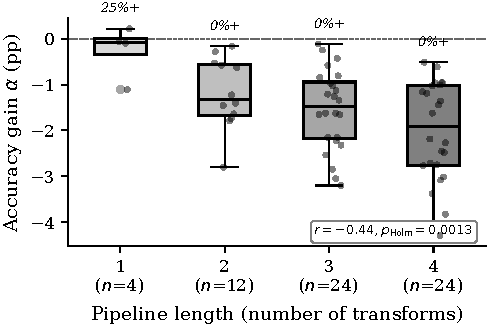
\includegraphics[width=\columnwidth]{fig_length_effect.pdf}
\caption{Distribution of accuracy gain ($\alpha$) by pipeline length across five seeds. The proportion of positive-$\alpha$ pipelines declines from 25\% at $k=1$ to 0\% at all longer lengths, and the overall length--$\alpha$ correlation is statistically significant after Holm--Bonferroni correction ($r = -0.44$, $p_{\text{Holm}} = 0.00132$).}
\label{fig:length_effect}
\end{figure}

\subsection{Variance Decomposition: Ordering Versus Selection}
\label{subsec:variance}

To quantify the relative contribution of transform selection versus transform ordering, the total variance in seed-averaged $\alpha$ among multi-stage pipelines was decomposed into a between-set component (attributable to which transforms are included) and a within-set component (attributable to how they are arranged) at each pipeline length. Pipelines sharing the same unordered set of transforms were grouped together, and a one-way ANOVA was computed with transform set as the grouping factor; residuals were checked for approximate normality via the Shapiro--Wilk test before ANOVA results were interpreted.

The variance decomposition is summarized in Fig.~\ref{fig:variance_decomp}. At $k=2$, each of the six transform pairs has two orderings. The seed-averaged point estimate attributes 76.1\% of variance to transform-set membership ($F(5,6)=3.81$, raw $p=0.067$; Shapiro--Wilk $p=0.74$). A 10{,}000-resample seed bootstrap gives $\eta^2$ CI $[0.57,0.90]$, but this interval is based on only five seed positions and does not replace the non-significant ANOVA. When all seed-level pipeline observations are pooled, $\eta^2$ falls to 0.22 because seed variation enters the residual. The $k=2$ selection share is therefore a descriptive point estimate, not a confirmed selection effect.

This relationship inverts at pipeline $k=3$, where each of the four possible transform triplets admits six orderings. The within-set (ordering) component accounts for 58\% of total variance, while the between-set (selection) component accounts for 42\% ($\eta^2 = 0.420$, $F(3,20) = 4.83$, raw $p = 0.0109$, $p_{\text{Holm}} = 0.0245$; Shapiro--Wilk $p = 0.99$). The selection effect is detectable in the full five-seed analysis but, as the leave-one-seed-out analysis below shows, is sensitive to seed exclusion.

At $k=4$, all 24 pipelines share the transform set $\{\text{E},\text{N},\text{D},\text{CS}\}$. Selection is constant by construction, so all observed configuration variance is within that set. The standard deviation is 1.07\,pp and the range is 3.78\,pp, from $-0.51$\,pp for D$\to$E$\to$CS$\to$N to $-4.29$\,pp for N$\to$D$\to$CS$\to$E. This range is about 2.8 times the 1.33\,pp spread across the four single-transform pipelines.

The progression from selection-dominated variance at $k=2$ to mixed selection--ordering contribution at $k=3$\footnote{The $k=3$ result is best read as suggestive evidence of a selection-to-ordering variance crossover rather than a categorical finding: the leave-one-seed-out analysis in Section~\ref{subsec:limitations} shows that the Holm-corrected significance of the length-3 ANOVA is sensitive to single-seed exclusion, losing corrected significance when seed~256 is removed.} to pure ordering variance at $k=4$ admits a combinatorial interpretation: with two transforms there are only two orderings per set, limiting the scope for ordering-induced divergence; with three transforms there are six orderings, and with four there are 24, providing increasingly many opportunities for detrimental arrangements to emerge.

\subsection{Transform Positional Preferences and the Bookend Structure}
\label{subsec:positional}

To investigate positional preferences, the seed-averaged mean $\alpha$ achieved by each transform was computed as a function of its ordinal position (first through fourth) across all pipelines in which it appears. This analysis, summarized in Fig.~\ref{fig:positional}, reveals a complementary pattern between equalization and normalization.

Equalization exhibits a monotonically deteriorating mean $\alpha$ as it is moved from position~1 to position~4 (from $-0.74$\,pp to $-3.12$\,pp), corresponding to a linear gradient of approximately $+0.78$\,pp per position toward the front. Normalization displays the mirror-image pattern (from $-2.25$\,pp at position~1 to $-0.91$\,pp at position~4), a gradient of approximately $+0.42$\,pp per position toward the end. Because later positions occur only in longer pipelines, Table~\ref{tab:positional} also reports within-length first-versus-last contrasts. The directions persist descriptively for equalization ($+0.40$, $+1.20$, and $+2.13$\,pp at $k=2,3,4$) and normalization ($-0.75$, $-1.22$, and $-1.91$\,pp), reducing but not eliminating concern about length composition. These contrasts share pipelines and seeds and should not be read as independent confirmatory tests.

To assess whether equalization's first-position advantage reflects a positional effect rather than a selection effect, two complementary permutation tests were run. The primary pooled test partitions the 64 non-baseline pipelines into equalization-first ($n = 16$) and all-others ($n = 48$, including 33 pipelines that contain equalization at a non-initial position and 15 that omit it); it yields a $+1.10$\,pp advantage with Cohen's $d = 1.22$ (raw $p = 0.00011$, $p_{\text{Holm}} = 0.00055$). Because that control blends omission with later placement, an exploratory within-inclusion test compared the 16 equalization-first pipelines only with the 33 pipelines containing equalization at a non-initial position. The contrast is $+1.22$\,pp ($d = 1.39$, raw $p = 0.00004$). The second result is not part of the primary Holm family, but its direction and magnitude show that omission alone does not explain the pooled contrast.

Denoising has a near-flat positional profile, with a gradient of approximately $-0.17$\,pp per position. Its descriptive within-length contrasts (Table~\ref{tab:positional}) are $-0.33$, $-0.39$, and $+0.13$\,pp at lengths 2, 3, and 4. Color-space conversion shows a weak negative gradient ($\approx -0.06$\,pp per position) in the pooled analysis, and its within-length contrasts ($+0.67$, $+0.41$, $-0.35$\,pp) change sign with length. Neither transform shows a consistent positional direction in these data.

\begin{table}[!t]
\caption{Within-length first-versus-last position contrasts for each transform (in percentage points of $\alpha$), controlling for the length-degradation confound. Positive $\Delta$ values indicate that the transform is less detrimental in first position than in last position. Equalization (E) shows a monotonically growing first-position advantage with length; normalization (N) shows a monotonically growing last-position advantage (negative $\Delta$); denoising (D) and color-space conversion (CS) show no consistent directional preference.\label{tab:positional}}
\centering
\footnotesize
\begin{tabular}{l r r r}
\toprule
\textbf{Transform} & \textbf{Length 2 ($\Delta$ pp)} & \textbf{Length 3 ($\Delta$ pp)} & \textbf{Length 4 ($\Delta$ pp)} \\
\midrule
E   & $+0.40$ & $+1.20$ & $+2.13$ \\
N   & $-0.75$ & $-1.22$ & $-1.91$ \\
D   & $-0.33$ & $-0.39$ & $+0.13$ \\
CS  & $+0.67$ & $+0.41$ & $-0.35$ \\
\bottomrule
\end{tabular}
\end{table}

The complementary positional structure is further examined by a bookend analysis of the first and last transforms. Pipelines adopting the equalization-first, normalization-last configuration ($n = 5$ across lengths 2--4) achieve a mean $\alpha$ of $-0.52$\,pp, compared with $-2.53$\,pp for the inverse configuration. The $+2.00$\,pp contrast is large (Cohen's $d = 2.38$) and remains significant after correction (raw $p = 0.0082$, $p_{\text{Holm}} = 0.0245$). In this experiment, the E--N bookend ordering minimizes harm rather than recovering a positive accuracy gain.

Because the two bookend arms are not uniformly distributed across lengths, the contrast was also computed within each length. Pipeline values were averaged within each arm at each seed, then the five paired seed differences were tested by exact sign flipping. The contrasts remain positive and large at $k=2$ ($+1.13$\,pp, $d = 1.86$), $k=3$ ($+1.90$\,pp, $d = 1.69$), and $k=4$ ($+2.55$\,pp, $d = 1.47$). All three exact two-sided tests yield $p = 0.0625$, the smallest attainable value above zero with five nonzero paired differences. These secondary results are directionally consistent with the pooled bookend contrast but do not independently reach the 0.05 level.

\begin{figure}[!ht]
\centering
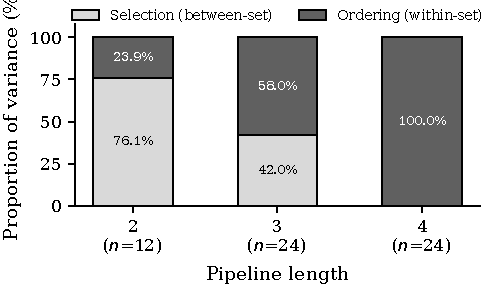
\includegraphics[width=\columnwidth]{fig_variance_decomp.pdf}
\caption{Variance decomposition across pipeline lengths. At $k=2$, transform selection accounts for $\eta^2 = 0.76$ of the variance (raw $p = 0.067$, not significant after correction). At $k=3$, ordering accounts for 58\% of the variance ($\eta^2_{\text{selection}} = 0.42$, $p_{\text{Holm}} = 0.0245$). At $k=4$, ordering is the sole source of variance by construction.}
\label{fig:variance_decomp}
\end{figure}

\begin{figure}[!t]
\centering
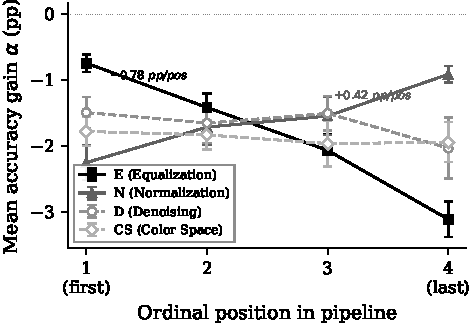
\includegraphics[width=\columnwidth]{fig_positional.pdf}
\caption{Mean $\alpha$ by ordinal position for each transform, averaged across five seeds with standard errors across pipelines containing each transform. Equalization (E) improves toward position~1 (gradient $\approx +0.78$\,pp/pos), and normalization (N) improves toward the final position (gradient $\approx +0.42$\,pp/pos). Denoising (D) and color-space conversion (CS) exhibit near-flat positional profiles.}
\label{fig:positional}
\end{figure}

\subsection{Fixed-Threshold Error Decomposition}
\label{subsec:error}

To describe how the two error counts change at the fixed decision threshold $\tau = 0.5$, the change in false positives ($\Delta\text{FP}$) and false negatives ($\Delta\text{FN}$) relative to the seed-matched baseline was computed for each pipeline and then averaged across seeds. Across the 64 non-baseline pipelines, the correlation between these changes is $r = +0.04$.

Fourteen pipelines (21.9\%) have opposite-sign changes: 10 increase false positives while decreasing false negatives, and four show the reverse. The remaining 50 pipelines (78.1\%) increase both error counts; none decreases both. This classification is a descriptive summary at one threshold. Without saved per-image scores, ROC curves, or calibration measurements, the sign pattern cannot distinguish a shifted operating point from a changed score distribution or establish irreversible feature loss.

\section{Discussion}
\label{sec:discussion}

\subsection{Ordering Effects in the Evaluated Implementation}

The 3.78\,pp range among the 24 length-4 pipelines shows that this CNN-plus-preprocessing implementation is sensitive to transform order. At $k=3$, within-set differences account for 58\% of the observed variance; at $k=4$, selection is constant by construction and all variation is among orderings. These results do not show that CNNs generally lack an invariance property. They show that the particular transform implementations and network used here did not absorb their order-dependent input changes.

The number of arrangements grows from two per transform set at $k=2$ to six at $k=3$ and 24 at $k=4$. This combinatorial growth increases the range of arrangements that can be evaluated, but it does not itself explain either the observed variance or the decline in mean $\alpha$. Empirically, arrangement affects the magnitude of harm in this experiment: no multi-transform pipeline has positive mean $\alpha$.

\subsection{Value-Range and Color-Space Contracts}
\label{subsec:mechanistic}

The order effects must be interpreted in light of the exact code. Images enter the pipeline as RGB tensors in $[0,1]$. Equalization and color-space conversion clamp their inputs to this interval. Normalization maps values by $(x-0.4)/0.2$, typically producing values outside $[0,1]$. Therefore, any later equalization or color conversion first discards out-of-range values through clamping. This deterministic range loss offers a direct implementation-level explanation for why normalization tends to perform better at the end and why equalization tends to perform better before normalization. It does not show that normalization destroys diagnostic information in general.

There is a second contract issue: RGB-to-HSV conversion produces hue in radians, whereas later transforms in this implementation treat any three-channel tensor as if it were RGB and may clamp it to $[0,1]$. Thus, pipelines that place another transform after color conversion can operate on semantically different channels or truncate hue values. The observed ordering effects consequently combine transform selection with domain and range mismatches. The harm-minimizing E-first/N-last pattern is specific to these implementations and parameters, not a universal transform-ordering rule.

\subsection{What the Confusion Matrices Establish}

At $\tau=0.5$, 78\% of non-baseline pipelines increase both false-positive and false-negative counts, while 22\% produce opposite-sign changes. This is useful for describing the deployed operating point, but not for identifying calibration error, ROC displacement, or feature-space damage. Those questions require saved per-image scores and threshold-independent evaluation. The present release contains only confusion matrices and accuracy summaries, so no claim about recovery by recalibration is made.

\subsection{Practical Implications}

For this near-ceiling binary task, the unprocessed baseline is best on average and no multi-transform pipeline improves mean accuracy. A practical lesson is therefore to validate whether preprocessing is needed before adding stages. If these exact transforms are required, the observed data favor placing equalization before normalization; the pooled bookend contrast is 2.00\,pp. Range-aware composition is at least as important as transform identity: every stage should document its expected input channels, numerical domain, and output domain, and conversions should be explicit.

Evaluating one conventional ordering does not characterize a transform set. When several non-commuting stages are used, alternative orderings should be tested or the composition should be redesigned so that all stages share compatible contracts. This recommendation concerns the evaluated software behavior and should be revalidated for other implementations and datasets.

\subsection{Limitations and Future Directions}
\label{subsec:limitations}

External validity is limited by one four-block CNN, one $128\times128$ binary task, one dataset pairing, four transforms, one parameter setting per transform, three training epochs, and five seeds. The transform parameters were fixed for the primary matrix. Historical exploratory searches used a different random image-level split and, for denoising, a different parameterization; they do not constitute independent tuning evidence. Parameter sensitivity therefore remains unmeasured.

The task is near ceiling ($\varepsilon_0=98.09\%$), bounding a possible positive gain to 1.91\,pp. The absence of multi-transform improvement should not be extrapolated to harder tasks. Five seeds are also too few for precise pipeline-specific inference: the reported bootstrap intervals are descriptive, and the within-length exact sign-flip tests have a minimum attainable two-sided $p$-value of 0.0625.

The most important internal-validity limitation is the construction of the label. Diseased images come from HAM10000, while healthy images come from a separate source. A linear model using spatially agnostic color moments reaches 93.4\% accuracy (AUROC 0.980), and color histograms reach 92.9\% (AUROC 0.980). The network can therefore exploit acquisition-source signatures that are strongly confounded with class. The experiment measures how preprocessing interacts with this combined source/class signal; it does not validate pathology discrimination or clinical utility. Replication should use both classes from a common acquisition process and an external test set.

The split is random at the image level, without stratification or lesion grouping. HAM10000 contains multiple images of some lesions~\cite{Tschandl2018}; consequently, related images may occur in different partitions. Future work should split by lesion identifier and report class counts per partition. Although a common split is used within each seed, model initialization and minibatch order are not paired across pipelines, so some between-pipeline differences also include optimization noise.

The leave-one-seed-out analysis supports the direction of the length, equalization-first, and pooled bookend results: the first two remain significant in all five exclusions, as does the pooled bookend test. The $k=3$ ANOVA is less stable, with corrected $p$-values ranging from 0.0033 to 0.0828, so the selection-to-ordering crossover should be considered suggestive. A larger number of seeds and a hierarchical analysis over matched seed-level contrasts would provide stronger uncertainty estimates.

Finally, the saved outputs do not contain per-image probabilities. AUROC, calibration, a decision-threshold sweep, and a valid same-image attribution comparison cannot be reconstructed without retraining. Future experiments should persist sample identifiers, logits, labels, and lesion groups; test range-safe transform implementations; and replicate across architectures, parameter settings, acquisition sites, and clinically meaningful endpoints.


\section{Conclusion}
\label{sec:conclusion}

This study exhaustively evaluates the 65 ordered pipelines formed from four preprocessing transforms, with five training seeds per pipeline. Pipeline length is negatively associated with mean accuracy gain ($r=-0.44$, $p_{\text{Holm}}=0.00132$), and no multi-transform pipeline improves on the 98.09\% mean baseline. Ordering accounts for 58\% of observed variance at $k=3$ and all variance at $k=4$ by construction. Equalization-first pipelines outperform the pooled alternatives ($d=1.22$, $p_{\text{Holm}}=0.00055$), and the equalization-first, normalization-last bookend differs from its reverse by 2.00\,pp ($d=2.38$, $p_{\text{Holm}}=0.0245$).

These findings describe one implementation on a strongly source-confounded, near-ceiling binary task. In particular, normalization produces values outside $[0,1]$, while later transforms clamp or reinterpret those values; the observed ordering pattern therefore partly reflects software range and color-space contracts. The result supports careful testing of transform composition and favors E-first/N-last as a harm-minimizing arrangement for this exact setup. It does not establish a universal ordering rule, clinical lesion discrimination, irreversible feature degradation, or recoverability by threshold calibration. Replication with lesion-grouped splits, a common acquisition source, range-safe transforms, saved per-image scores, more seeds, and additional architectures is required.


\section*{Funding}
The research reported here did not receive any specific grant from funding agencies in the public, commercial, or not-for-profit sectors. If this article is accepted for publication, its open-access article publishing charge will be covered by the Coordena\c{c}\~ao de Aperfei\c{c}oamento de Pessoal de N\'ivel Superior (CAPES), Brazil.


\section*{CRediT authorship contribution statement}
\textbf{Gabriel Mitelman Tkacz}: Conceptualization, Methodology, Software, Validation, Formal analysis, Investigation, Data curation, Writing -- original draft, Writing -- review \& editing, Visualization. \\
\textbf{Gustavo Scalabrini Sampaio}: Conceptualization, Supervision, Writing -- review \& editing, Project administration. \\
\textbf{Leandro Augusto da Silva}: Conceptualization, Supervision, Writing -- review \& editing, Project administration.


\section*{Declaration of competing interest}
The authors declare that they have no known competing financial interests or personal relationships that could have appeared to influence the work reported in this paper.


\section*{Ethics statement}
This study is a secondary computational analysis of publicly available, de-identified image datasets. No new participant data were collected, the authors had no access to direct identifiers, and no participant contact or intervention occurred. Accordingly, no new ethics approval or informed consent was required for this analysis.


\section*{Declaration of generative AI and AI-assisted technologies in the writing process}
During the preparation of this work the authors used Anthropic Claude and OpenAI Codex to support literature cross-checking, code review, prose editing, and LaTeX formatting. After using these tools, the authors reviewed and edited the content as needed and take full responsibility for the content of the publication.


\section*{Data availability}
The HAM10000 dataset is publicly available via the ISIC Archive and the Harvard Dataverse~\cite{Tschandl2018}. The healthy-skin images used to construct the negative class are drawn from the publicly available Healthy Skin Dataset distributed via Hugging Face~\cite{megpaulson_healthy_skin}. Training and analysis code, the exact dataset checksum manifest, per-seed confusion matrices, and the aggregated analysis are provided at \url{https://github.com/gtkacz/undergrad_thesis}. Per-image model scores were not retained and are therefore unavailable. The five random seeds used in this study are $\{42, 123, 256, 512, 1024\}$.

\bibliographystyle{elsarticle-num}
\bibliography{refs}

\end{document}
